\section{Introduction}

As a free online service, VirusTotal~\cite{virustotal} analyzes files submitted by real-world users to identify many different kinds of malwares, 
like viruses, worms, trojans, and so on. 
VirusTotal applies different antivirus engines to each submitted file and generate an aggregated reports. 
All submitted files and generated reports are saved and can be accessed through VirusTotal’s API. 
Inspired by previous mining software repositories~\cite{GuoICSE2010,bigcode, big-lessons,big-translation,code-completion,big-predicting} 
work in software engineer and programming languages community, 
we believe leveraging data on VirusTotal could enable many ``big security'' applications.  

The repository on VirusTotal provides a valuable source to conduct data mining. 
Firstly, there are huge amount of data on VirusTotal.
Figure~\ref{fig:subnum} shows that there were more than 40 million suspicious files 
submitted in November of 2015. 
This amount of data makes VirusTotal a rough estimation of malwares in the real world. 
Secondly, all data on VirusTotal are labeled by state-of-the-art antivirus techniques. 
VirusTotal updates each antivirus engine every 5 minutes. 
Besides whether a given a submitted file is detected by an antivirus engine, VirusTotal also keeps exact detection tag returned by each engine. 
There are also online active malware researchers, 
who can comment and vote each submitted file 
and serve as an important supplement of antivirus engines. 

In industry, antivirus vendors widely use VirusTotal to identify false negatives 
and false positives in their products. 
They only utilize VirusTotal reports separately for each single suspicious file, 
but fail to consider correlations among different suspicious files. 
In academia, researchers began to pay attention to mining VirusTotal repository. 
For example, ~\citet{neeles} leverage submission\_id information to identify malware writers, 
who use VirusTotal as a test platform. 
We believe there are much more research opportunities through mining VirusTotal. 

In this paper, we conduct an empirical study on malware dataset on VirusTotal. 
An empirical study is the prerequisite to conduct data mining on VirusTotal. 
We first collect more than 40 million suspicious file submissions on VirusTotal, and then 
we focus our analysis on Windows executable and binary malwares detected Microsoft
antivirus engine to guarantee accuracy. 
Our analysis begins from general characteristics, such as submission frequency and the generation rate of malware families. 
We then specifically look into the temporal characteristic and family distribution characteristic. 
We hypothesize that malwares do not appear uniformly across time, and they appear in bursts. 
To validate our hypothesis, we build a cache-based malware prediction technique, which aims to predict malwares in which family would appear in the near future. 
Our malware family cache can achieve 90\% cache hit rates by only using 100 cache entries.
Our technique would allow antivirus vendors to focus their effort. 
We observe the distribution of malware families is highly skewed. 
We view malware submissions as a stream, based on their submission timestamp, and apply a frequent item mining algorithm to identify hot malware families. 
Our solution can precisely answer hot malware family query in nearly-real time, by using a constant number of counters. 


\begin{figure}[t!]
\begin{center}
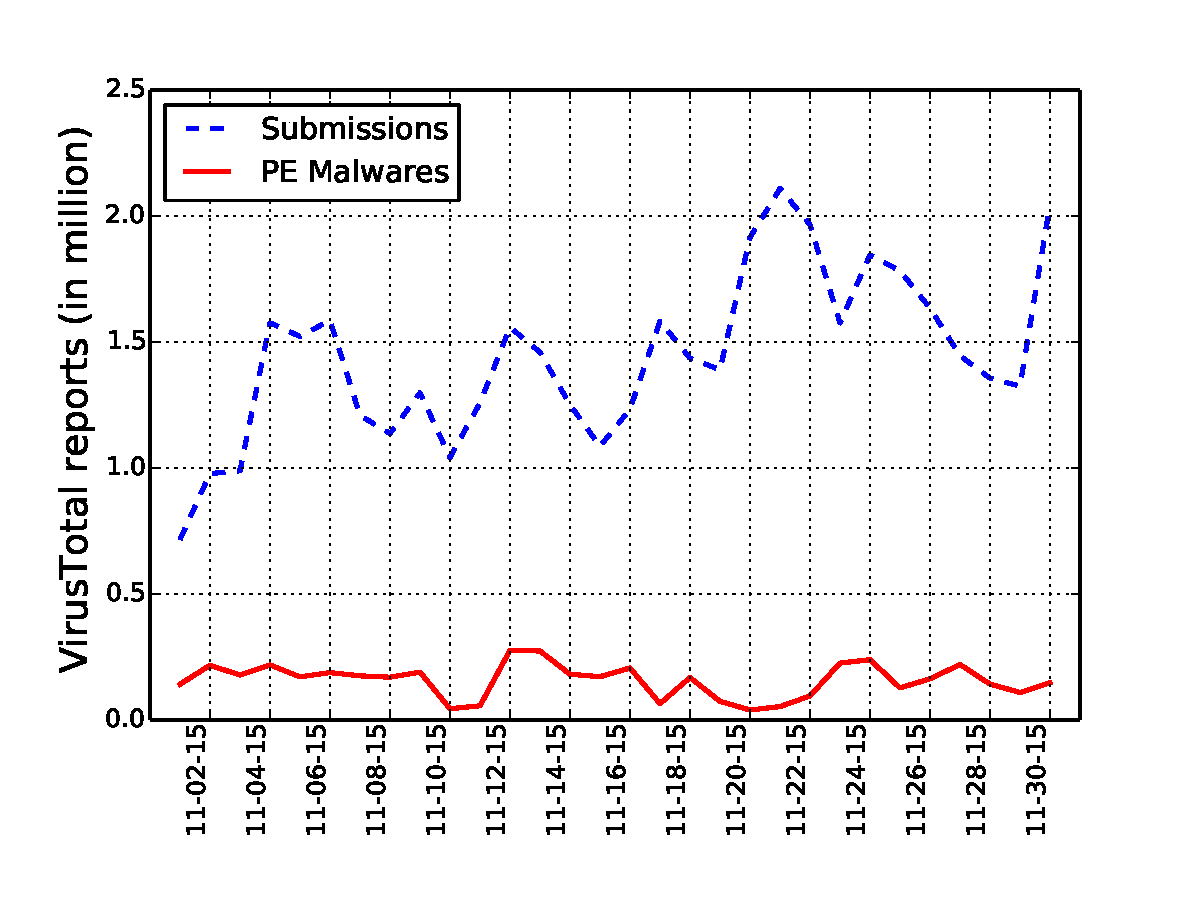
\includegraphics[width=3.3in]{figure/nov}
\caption{The number of suspicious files and the number of malwares submitted to VirusTotal in November of 2015. }
\label{fig:subnum}
\end{center}
\end{figure}

To sum up, we made the following contributions in this paper:

\begin{itemize}

\item We collect data submitted to VirusTotal in November of 2015, 
and analyze their general characteristics. 
We find that most malware samples are only submitted once to VirusTotal, 
and roughly 100-400 malware families appear each day~\ref{sec:label}. 

\item We hypothesize that malwares appear in bursts. 
Our cache-based malware prediction technique confirms our hypothesis, 
and it can achieve more 90\% prediction precision~\ref{sec:predict}. 

\item We observe that family distributions of malwares are highly skewed. 
Leveraging this observation, we build a hot malware family mining solution, 
which can identify hot malware families by using a constant number of counters~\ref{sec:distribution}

\item We discuss the future research opportunities through mining data on VirusTotal~\label{sec:oppo}. 

\end{itemize}


